\documentclass{beamer}
\usepackage{graphicx}
\usetheme{Berlin}

\title{FYP Week3 Review}
\subtitle{Using Beamer}
\author{Lenox Low}
\institute{Multimedia University Cyberjaya Campus}
\date{\today}

\begin{document}

\begin{frame}
\titlepage
\end{frame}

\begin{frame}
\frametitle{Outline}
\tableofcontents
\end{frame}

\section{Research Paper Reading}
\subsection{X Mean}

\begin{frame}
\frametitle{X-Mean - Introduction}
It is an algorithm that able to search the space of the cluster locations efficiently and the optimal number of clusters (the value of K). The Bayesian Information Criterion (BIC) or Akaike Information Criterion (AIC) measurement is used for determining the value of K. 

\end{frame}

\begin{frame}
\frametitle{X-Mean - Procedures}
It goes into action after each run of K-means, making local decisions about which subset of the current centroids should split themselves in order to better fit the data. The splitting decision is done by computing the Bayesian Information Criterion.
\end{frame}

\begin{frame}
\frametitle{X-Mean Procedures(Cont.)}
\begin{figure}[hbt!]\centering
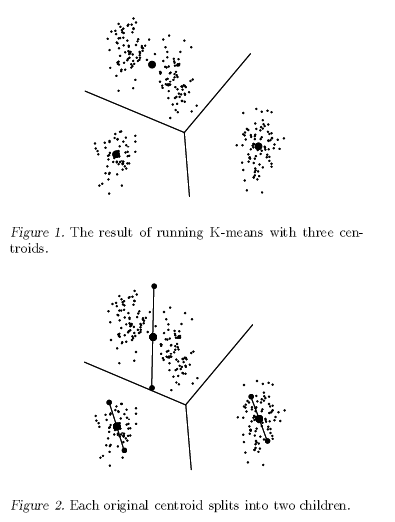
\includegraphics[scale=0.3]{image/xmean1}
\end{figure}
\end{frame}

\begin{frame}
\frametitle{X-Mean Procedures(Cont.)}
\begin{figure}[hbt!]\centering
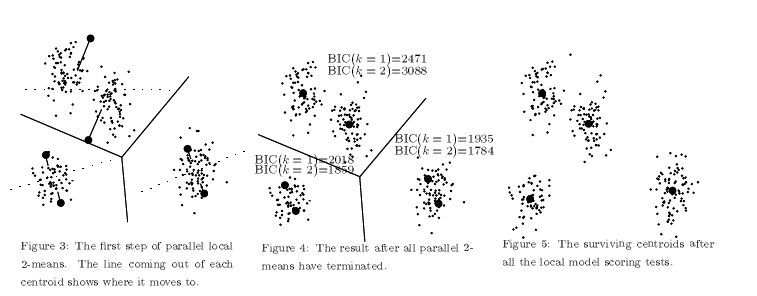
\includegraphics[scale=0.4]{image/xmean2}
\end{figure}
\end{frame}

\section{FYP Steps}
\subsection{FYP Step I}
\begin{frame}
\frametitle{Data Collection}
\begin{itemize}
\item Few features is selected and collected using Torque(Lite)
\item Currently 9 drivers file is available.
\end{itemize}
\end{frame}

\begin{frame}
\frametitle{Data Collection (Cont.)}
The features include
\begin{itemize}
\item GPS coordinate
\item Speed (GPS)
\item GPS Bearing
\item GPS Altitude
\item Engine RPM
\item Engine Load
\item Throttle Position
\item Engine Coolant Temperature
\item Acceleration Sensor (Total)
\end{itemize}
\end{frame}

\subsection{FYP Step II}
\begin{frame}
\frametitle{Data Preprocessing}
\begin{itemize}
\item Eliminate the first few rows and last few few rows of the data.
\item Road Structure Labelling
	\begin{enumerate}
	\item Manual label the road structure of a single data set using Google Earth
	\item Develop scripts to label the remaining data sets using Python
	\item Check the result of the scripts using the Tableau.
	\end{enumerate}

\item Data Fusion
\end{itemize}
\end{frame}

\subsection{FYP Step III}
\begin{frame}
\frametitle{Data Exploring}
\begin{itemize}
\item Explore the data distribution by using K Means Algorithm
\item Find the optimal number of clusters (The result is 2)
\end{itemize}
\end{frame}

\subsection{FYP Step IV}
\begin{frame}
\frametitle{Driver Profiling}
Propose method
\end{frame}

\subsection{FYP Step V}
\begin{frame}
\frametitle{Data Classification}
Naive Bayes will be used as Machine Learning Technique to train the classifier
\end{frame}

\begin{frame}
Thank you
\end{frame}

\end{document}


